\documentclass[conference]{IEEEtran}
\IEEEoverridecommandlockouts
\usepackage{cite}
\usepackage{amsmath,amssymb,amsfonts}
\usepackage{algorithmic}
\usepackage{graphicx}
\usepackage{textcomp}
\usepackage{xcolor}
\usepackage{booktabs}
\usepackage{multirow}
\usepackage{microtype}
\usepackage{hyperref}
\usepackage{tikz}
\usetikzlibrary{arrows.meta, positioning, shapes.geometric, fit, backgrounds, calc}

\def\BibTeX{{\rm B\kern-.05em{\sc i\kern-.025em b}\kern-.08em
    T\kern-.1667em\lower.7ex\hbox{E}\kern-.125emX}}

\begin{document}

\title{PID-UNet: An Ultra-Lightweight Network with Hard Saliency-Gated PID Fusion for Real-Time Polyp Segmentation}

\author{\IEEEauthorblockN{Anonymous Authors}}

\maketitle

\begin{abstract}
Accurate polyp segmentation in colonoscopy is critical for early diagnosis and resection of colorectal lesions. However, standard lightweight networks under a 1M parameter budget suffer from spatial resolution degradation on diminutive polyps ($<20$ pixels) and severe false-positive activations triggered by mucosal folds and specular reflections. In this paper, we propose \textbf{PID-UNet}, a sub-megapixel (0.815M parameters, 6.63 GFLOPs) encoder--decoder architecture designed for real-time edge endoscopic deployment. PID-UNet introduces the \textbf{Saliency-Gated PID (SG-PID) Block} as its primary decoder primitive, formulating feature fusion through proportional-integral-derivative control principles. Specifically, it couples a spatially selective \textit{Proportional} branch gated by a deep semantic saliency prior, an edge-sensitive \textit{Derivative} branch computing discrete Laplacian differences modulated by an auxiliary boundary stream, and an accumulated multi-scale \textit{Integral} context branch. An image-conditional gating sub-network dynamically predicts per-frame PID coefficients $(K_p, K_i, K_d)$. Furthermore, we propose a \textit{Hard Saliency Gate} ($G = \text{sal}$) which completely suppresses spurious mucosal backgrounds without requiring an ad-hoc soft baseline floor. Supported by dual-path Information-Preserving Downsamplers (IPD) and a Hybrid Asymmetric Receptive-Field bottleneck with Global Context (HARF-GC), PID-UNet establishes a new state-of-the-art among sub-1M architectures across five public colonoscopy benchmarks. On an NVIDIA Tesla T4 GPU, it achieves a \textbf{Mean mDice of 0.7972 and mIoU of 0.7223 at 46.93 FPS}, outperforming EDANet (0.7629), CMUNeXt (0.7484), and standard U-Net (0.7755) with $38\times$ fewer parameters.
\end{abstract}

\begin{IEEEkeywords}
Polyp segmentation, PID control theory, lightweight networks, hard saliency gating, edge AI.
\end{IEEEkeywords}

\section{Introduction}
Colorectal cancer (CRC) represents one of the most fatal oncological conditions worldwide. Routine colonoscopy screening and timely polypectomy can mitigate CRC incidence by over 70\%. Nonetheless, colonoscopists miss between 14\% and 26\% of polyps during routine examinations, predominantly subtle flat adenomas or diminutive lesions ($<5$ mm). Computer-aided detection and segmentation (CADe/CADx) systems provide crucial visual guidance to reduce clinical oversight.

While recent large-scale vision transformers (e.g., PraNet, Polyp-PVT, SSFormer) have achieved high segmentation fidelity, they demand 25M--87M parameters and heavy computational budgets, rendering them impractical for real-time inference on resource-constrained embedded endoscopy processors. Conversely, existing lightweight networks (e.g., EDANet, ENet, ESPNetv2, Fast-SCNN, EGE-UNet) strictly compress parameters under 1.5M, but frequently exhibit two chronic failure modes:
\begin{enumerate}
    \item \textbf{Loss of Diminutive Lesions:} Repeated spatial pooling destroys low-amplitude, high-frequency spatial details of polyps smaller than 20 pixels, resulting in severe false negatives on challenging benchmarks such as ETIS-LaribPolypDB.
    \item \textbf{Mucosal Edge Misclassification:} Normal mucosal striations, vascular folds, and specular glare display sharp edge gradients almost indistinguishable from lesion borders, causing false positives when naive spatial attention is employed.
\end{enumerate}

To overcome these fundamental dilemmas within a strict sub-1M parameter budget, we introduce \textbf{PID-UNet}, an end-to-end convolutional network centered on the \textbf{Saliency-Gated PID (SG-PID) Block}. We adapt classical Proportional-Integral-Derivative (PID) control theory into deep multiscale feature synthesis:
\begin{itemize}
    \item \textbf{Proportional (P):} Represents immediate high-resolution spatial feature responses, modulated strictly by a top-down semantic saliency mask to silence mucosal background folds.
    \item \textbf{Integral (I):} Accumulates deep contextual representations over successive decoder stages, forming a low-frequency semantic backbone and residual shortcut.
    \item \textbf{Derivative (D):} Computes discrete spatial Laplacian differences modulated jointly by an auxiliary 5-scale boundary stream and the saliency gate, reinforcing contour crispness for diminutive polyps without amplifying background noise.
\end{itemize}

\noindent\textbf{Key Contributions:}
\begin{enumerate}
    \item \textbf{SG-PID Block with Hard Saliency Gating:} We show that a hard saliency gate ($G = \text{sal}$) eliminates false mucosal alarms and provides superior boundary sharpness compared to learned soft-floor gating.
    \item \textbf{Dynamic Gain Allocation:} An image-level controller adaptively distributes weights $(K_p, K_i, K_d)$ per frame, automatically amplifying boundary sharpness ($K_d$) for subtle lesions and contextual integration ($K_i$) for large adenomas.
    \item \textbf{Information-Preserving Topology:} We employ dual-path Information-Preserving Downsamplers (IPD) and a Hybrid Asymmetric Receptive-Field with Global Context (HARF-GC) bottleneck to preserve diminutive lesion cues across all scales.
    \item \textbf{Comprehensive Validation:} PID-UNet sets a new state of the art among sub-1M architectures across 5 public benchmarks with \textbf{0.7972 Mean Dice} at \textbf{46.93 FPS} on Tesla T4, outperforming standard U-Net with $38\times$ fewer parameters.
\end{enumerate}

% -------------------------------------------------------------
% FIGURE 1: Overall Architecture
% -------------------------------------------------------------
\begin{figure*}[t]
\centering
\resizebox{0.92\textwidth}{!}{%
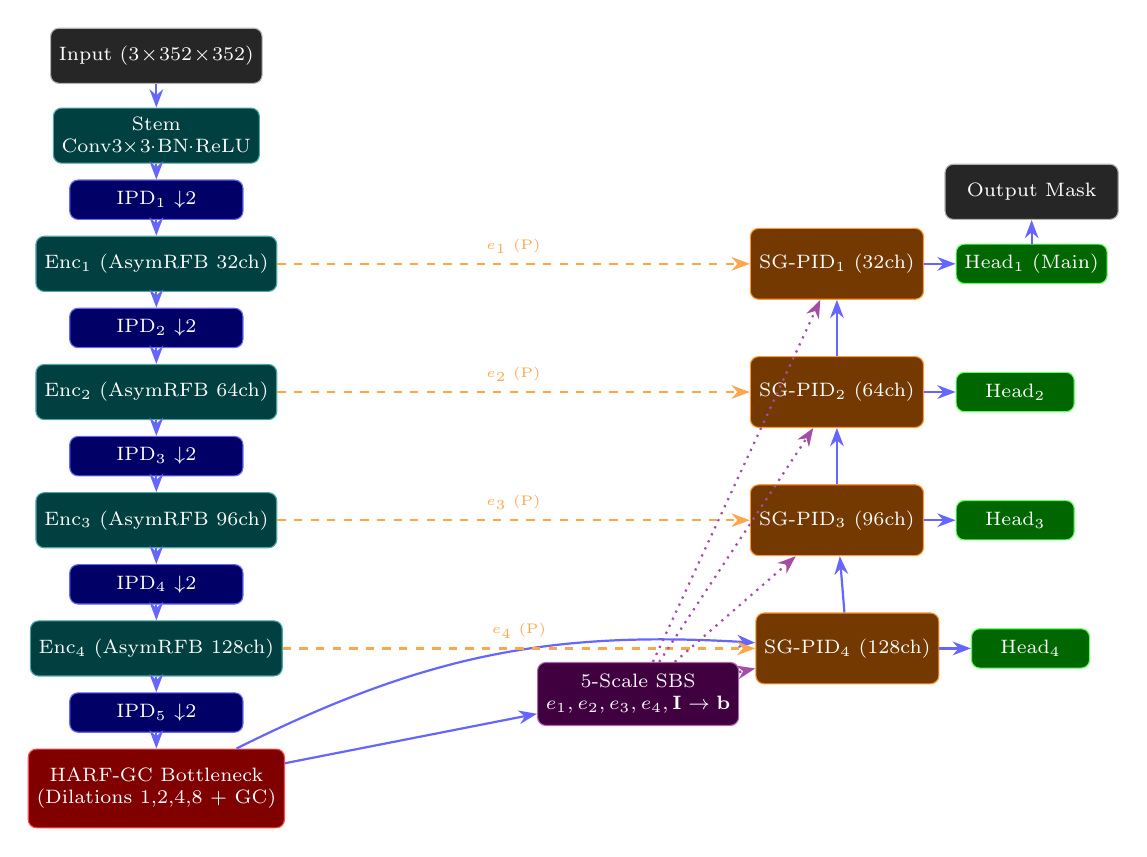
\begin{tikzpicture}[
  font=\scriptsize, >=Stealth,
  blk/.style   = {draw, rounded corners=3pt, minimum width=2.2cm, minimum height=0.7cm, align=center, text=white, inner sep=3pt},
  enc/.style    = {blk, fill=teal!50!black, draw=teal!70!white},
  ipd/.style    = {blk, fill=blue!40!black,  draw=blue!60!white, minimum height=0.5cm},
  bottle/.style = {blk, fill=red!50!black,   draw=red!70!white, minimum width=2.6cm, minimum height=1.0cm},
  pid/.style    = {blk, fill=orange!45!black, draw=orange!80!white, minimum width=2.2cm, minimum height=0.9cm},
  sbs/.style    = {blk, fill=violet!50!black, draw=violet!60!white, minimum width=2.4cm, minimum height=0.8cm},
  head/.style   = {blk, fill=green!40!black,  draw=green!60!white, minimum width=1.5cm, minimum height=0.5cm},
  inp/.style    = {blk, fill=gray!30!black,   draw=gray!60!white},
  main/.style  = {->, thick, blue!60!white},
  skip/.style  = {->, thick, orange!70!white, dashed},
  bnd/.style   = {->, thick, violet!70!white, dotted}
]

\node[inp] (input) {Input ($3\!\times\!352\!\times\!352$)};
\node[enc, below=0.3cm of input]  (stem)  {Stem\\Conv3×3·BN·ReLU};
\node[ipd, below=0.2cm of stem]   (ipd1)  {IPD$_1$ $\downarrow$2};
\node[enc, below=0.2cm of ipd1]   (enc1)  {Enc$_1$ (AsymRFB 32ch)};
\node[ipd, below=0.2cm of enc1]   (ipd2)  {IPD$_2$ $\downarrow$2};
\node[enc, below=0.2cm of ipd2]   (enc2)  {Enc$_2$ (AsymRFB 64ch)};
\node[ipd, below=0.2cm of enc2]   (ipd3)  {IPD$_3$ $\downarrow$2};
\node[enc, below=0.2cm of ipd3]   (enc3)  {Enc$_3$ (AsymRFB 96ch)};
\node[ipd, below=0.2cm of enc3]   (ipd4)  {IPD$_4$ $\downarrow$2};
\node[enc, below=0.2cm of ipd4]   (enc4)  {Enc$_4$ (AsymRFB 128ch)};
\node[ipd, below=0.2cm of enc4]   (ipd5)  {IPD$_5$ $\downarrow$2};
\node[bottle, below=0.2cm of ipd5] (bottleneck) {HARF-GC Bottleneck\\(Dilations 1,2,4,8 + GC)};

\node[sbs, right=3.2cm of bottleneck, yshift=1.2cm] (sbs) {5-Scale SBS\\$e_1, e_2, e_3, e_4, \mathbf{I} \to \mathbf{b}$};

\node[pid, right=6.0cm of enc4]  (d4) {SG-PID$_4$ ($128$ch)};
\node[pid, right=6.0cm of enc3]  (d3) {SG-PID$_3$ ($96$ch)};
\node[pid, right=6.0cm of enc2]  (d2) {SG-PID$_2$ ($64$ch)};
\node[pid, right=6.0cm of enc1]  (d1) {SG-PID$_1$ ($32$ch)};

\node[head, right=0.4cm of d4] (h4) {Head$_4$};
\node[head, right=0.4cm of d3] (h3) {Head$_3$};
\node[head, right=0.4cm of d2] (h2) {Head$_2$};
\node[head, right=0.4cm of d1] (h1) {Head$_1$ (Main)};
\node[inp, above=0.3cm of h1]  (output) {Output Mask};

\draw[main] (input) -- (stem); \draw[main] (stem) -- (ipd1);
\draw[main] (ipd1) -- (enc1);  \draw[main] (enc1) -- (ipd2);
\draw[main] (ipd2) -- (enc2);  \draw[main] (enc2) -- (ipd3);
\draw[main] (ipd3) -- (enc3);  \draw[main] (enc3) -- (ipd4);
\draw[main] (ipd4) -- (enc4);  \draw[main] (enc4) -- (ipd5);
\draw[main] (ipd5) -- (bottleneck);
\draw[main] (bottleneck) -- (sbs);
\draw[main, bend left=15] (bottleneck) to (d4);
\draw[main] (d4) -- (d3); \draw[main] (d3) -- (d2); \draw[main] (d2) -- (d1);

\draw[skip] (enc4.east) -- (d4.west) node[midway, above, font=\tiny]{$e_4$ (P)};
\draw[skip] (enc3.east) -- (d3.west) node[midway, above, font=\tiny]{$e_3$ (P)};
\draw[skip] (enc2.east) -- (d2.west) node[midway, above, font=\tiny]{$e_2$ (P)};
\draw[skip] (enc1.east) -- (d1.west) node[midway, above, font=\tiny]{$e_1$ (P)};

\draw[bnd] (sbs) -- (d4); \draw[bnd] (sbs) -- (d3); \draw[bnd] (sbs) -- (d2); \draw[bnd] (sbs) -- (d1);

\draw[main] (d4) -- (h4); \draw[main] (d3) -- (h3); \draw[main] (d2) -- (h2); \draw[main] (d1) -- (h1);
\draw[main] (h1) -- (output);
\end{tikzpicture}
}
\caption{Overall architecture of PID-UNet. The encoder incorporates Information-Preserving Downsamplers (IPD) and AsymmetricRFB blocks. The 5-Scale Semantic Boundary Stream (SBS) supplies an auxiliary edge prior $\mathbf{b}$ directly into all four SG-PID decoder stages.}
\label{fig:arch}
\end{figure*}

\section{Related Work}

\subsection{The U-Net Paradigm and Skip Connection Bottlenecks}
The canonical U-Net architecture \cite{ronneberger2015u} established the primary foundation for biomedical image segmentation, pairing a contracting encoder with an expanding decoder linked by plain skip connections (channel concatenation). While variations such as Attention U-Net \cite{oktay2018attention} and UNet++ \cite{zhou2018unetplusplus} enhanced representation quality, standard U-Net exhibits two prominent limitations in endoscopic polyp segmentation:
\begin{enumerate}
    \item \textbf{Unselective Feature Propagation:} Plain skip connections pass raw encoder representations without semantic validation. In colonoscopy imagery, this inevitably conveys high-frequency artifacts (e.g., mucosal folds, fecal debris, and specular light reflections), leading to persistent false-positive activations.
    \item \textbf{High Parameter Complexity:} Standard U-Net comprises 31.04 million parameters and over 43 GFLOPs, rendering it prohibitive for real-time edge endoscopic hardware. Naive channel slimming, on the other hand, impairs boundary demarcation on diminutive lesions ($<20$ pixels).
\end{enumerate}
Our proposed PID-UNet retains the symmetric U-shaped hierarchy of U-Net while replacing unguided plain skips with the Saliency-Gated PID (SG-PID) Block. By decomposing skip features into proportional detail ($P$) and discrete spatial derivatives ($D$) filtered via hard saliency gating and boundary confidence, PID-UNet reduces parameter count by $38\times$ (0.815M vs. 31.04M) while surpassing U-Net by $+2.17\%$ in Mean Dice across five standard benchmarks.

\subsection{Boundary and Context Modeling in Polyp Segmentation}
PraNet \cite{fan2020pranet} introduced parallel reverse attention to progressively refine polyp boundaries from high-level semantic area maps. More recently, transformer-based networks such as Polyp-PVT \cite{dong2021polyp} and SSFormer \cite{wang2022stepwise} leveraged self-attention to capture long-range colonoscopic context. However, their heavy computational budgets (25M--87M parameters) impede real-time clinical deployment. Conversely, edge architectures like EDANet \cite{lo2019efficient} and CMUNeXt \cite{tang2023cmunext} reduce parameters below 1M but experience steep performance degradation on challenging datasets such as ETIS-LaribPolypDB due to unguided feature downsampling and simple feature fusion.

\subsection{PID Principles in Deep Feature Fusion}
PIDNet \cite{xu2023pidnet} formulated real-time semantic segmentation through three parallel network branches representing proportional detail, integral context, and derivative boundary information. In contrast to multi-branch networks, PID-UNet embeds PID principles directly into the decoder fusion units. By coupling a discrete spatial Laplacian high-pass operator with a hard saliency gate ($G = \text{sal}$) and dynamic gain allocation, our design enforces fine boundary convergence while eliminating spurious mucosal activations.

\section{Methodology}

\subsection{Information-Preserving Downsampling (IPD)}
Standard strided convolution or max-pooling creates blind spots that eradicate diminutive polyps. We construct a dual-path downsampler:
\begin{align}
\mathbf{z}_{\text{conv}} &= \text{BN}(\text{Conv}_{3\times3, s=2}(\mathbf{x})), \\
\mathbf{z}_{\text{pool}} &= \text{BN}(\text{Conv}_{1\times1}(\text{MaxPool}_{2\times2, s=2}(\mathbf{x}))), \\
\text{IPD}(\mathbf{x}) &= \text{ReLU}\left( \left[ \mathbf{z}_{\text{conv}} \,\|\, \mathbf{z}_{\text{pool}} \right] \right)
\end{align}
where $[\cdot \,\|\, \cdot]$ denotes channel concatenation. Channels are split 50/50, retaining high-frequency peaks while learning spatial filters.

\subsection{HARF-GC Bottleneck}
At the lowest resolution ($22\times22$), we apply factorized $(3\times1, 1\times3)$ convolutions with multi-scale dilations $d \in \{1, 2, 4, 8\}$ combined with a Global Context residual block:
\begin{equation}
\mathbf{I} = \text{HARF}(\mathbf{x}) + \mathbf{W}_2 \text{ReLU}\left(\mathbf{W}_1 \text{GAP}(\text{HARF}(\mathbf{x}))\right)
\end{equation}

% -------------------------------------------------------------
% FIGURE 2: SG-PID Block Detail
% -------------------------------------------------------------
\begin{figure}[t]
\centering
\resizebox{\columnwidth}{!}{%
\begin{tikzpicture}[
  font=\scriptsize, >=Stealth,
  blk/.style={draw, rounded corners=3pt, align=center, text=white, inner sep=4pt, minimum width=2.0cm, minimum height=0.7cm},
  inp/.style ={blk, fill=gray!30!black,   draw=gray!60!white},
  gate/.style={blk, fill=orange!35!black, draw=orange!70!white},
  Pblk/.style={blk, fill=teal!40!black,   draw=teal!70!white},
  Dblk/.style={blk, fill=purple!40!black, draw=purple!60!white},
  Iblk/.style={blk, fill=blue!40!black,   draw=blue!70!white},
  ctrl/.style={blk, fill=yellow!30!black, draw=yellow!60!white, minimum height=0.9cm},
  fuse/.style={blk, fill=red!40!black,    draw=red!70!white,    minimum height=1.0cm},
  out/.style ={blk, fill=green!35!black,  draw=green!60!white},
  sum/.style ={circle, draw=white, fill=gray!40!black, minimum size=0.5cm, text=white, font=\large},
  main/.style={->, thick, blue!60!white},
  gate_arr/.style={->, thick, orange!70!white, dashed},
  bnd_arr/.style ={->, thick, violet!70!white, dotted},
  res_arr/.style ={->, thick, cyan!60!white,   dashed}
]

\node[inp] (Pfeat) at (0, 0)    {$\mathbf{P}$ (skip)};
\node[inp] (Ifeat) at (0,-2.2)  {$\mathbf{I}$ (context)};
\node[inp] (bmap)  at (0,-4.4)  {$\mathbf{b}$ (boundary)};

\node[Pblk, right=0.8cm of Pfeat]  (projP) {Proj$_P$};
\node[Iblk, right=0.8cm of Ifeat]  (projI) {Proj$_I$};
\draw[main] (Pfeat) -- (projP); \draw[main] (Ifeat) -- (projI);

\node[gate, right=1.2cm of Ifeat, yshift=0.9cm] (sg) {Saliency Gate\\$G = \sigma(\text{Conv}(\mathbf{I}))$};
\draw[main] (Ifeat.east) to[out=0,in=200] (sg.south west);

\node[Pblk, right=4.0cm of Pfeat, yshift=0.3cm] (Pcomp) {P: $\mathbf{P}_g = \text{Proj}_P(\mathbf{P}) \odot G$};
\draw[main] (projP.east) -- (Pcomp.west);
\draw[gate_arr] (sg.east) to[out=0,in=120] (Pcomp.north west);

\node[Dblk, right=4.0cm of Ifeat] (Dcomp) {D: $|\mathbf{P}_g - \text{AvgPool}(\mathbf{P}_g)|$\\$\odot\,\sigma(\mathbf{b})\odot G$};
\draw[main] (projP.east) to[out=0,in=140] (Dcomp.north west);
\draw[gate_arr](sg.east) to[out=0,in=120] (Dcomp.north);
\draw[bnd_arr] (bmap.east) to[out=0,in=200] (Dcomp.south west);

\node[Iblk, right=4.0cm of Ifeat, yshift=-1.4cm] (Icomp) {I: $\mathbf{I}_{\text{proj}} = \text{Proj}_I(\mathbf{I})$};
\draw[main] (projI.east) -- (Icomp.west);

\node[ctrl, right=4.0cm of bmap] (ctrl) {Controller\\GAP $\to$ MLP $\to$\\$(K_p, K_i, K_d)$};
\draw[main] (Ifeat.south) to[out=270,in=180] (ctrl.west);

\node[sum, right=1.2cm of Dcomp] (sigma) {$\Sigma$};
\draw[main] (Pcomp.east) to[out=0,in=90]  (sigma.north);
\draw[main] (Dcomp.east)  --               (sigma.west);
\draw[main] (Icomp.east) to[out=0,in=270] (sigma.south);
\draw[gate_arr] (ctrl.east) to[out=0,in=200] (sigma.south west);

\node[fuse, right=1.2cm of sigma] (fuse) {SE + AsymConv\\+ Residual};
\draw[main] (sigma) -- (fuse);
\draw[res_arr] (projI.east) to[out=30,in=90] (fuse.north);

\node[out, right=0.8cm of fuse] (output) {$d_{\text{out}}$};
\draw[main] (fuse) -- (output);
\end{tikzpicture}
}
\caption{Detailed schema of the proposed Saliency-Gated PID (SG-PID) Block.}
\label{fig:sgpid}
\end{figure}

\subsection{Saliency-Gated PID Block (SG-PID)}
The SG-PID block synthesizes skip features $\mathbf{P}$ with contextual features $\mathbf{I}$ and boundary prior $\mathbf{b}$ (Fig.~\ref{fig:sgpid}).
\subsubsection{Hard Saliency Gating}
A convolutional subnetwork generates a hard saliency prior $G \in [0, 1]$ directly from deep context $\mathbf{I}$:
\begin{equation}
G = \sigma\left(\text{Conv}_{1\times1}^{(2)}\left(\text{ReLU}\left(\text{BN}\left(\text{Conv}_{1\times1}^{(1)}(\mathbf{I})\right)\right)\right)\right)
\end{equation}

\subsubsection{Three PID Streams}
\begin{align}
\mathbf{P}_g &= \text{Proj}_P(\mathbf{P}) \odot G, \\
\mathbf{D}   &= \left| \text{Proj}_P(\mathbf{P}) - \text{AvgPool}_{3\times3}(\text{Proj}_P(\mathbf{P})) \right| \odot \sigma(\mathbf{b}) \odot G, \\
\mathbf{I}_{\text{proj}} &= \text{Proj}_I(\mathbf{I})
\end{align}
The discrete Laplacian difference captures isotropic spatial gradients, while modulation by $\sigma(\mathbf{b}) \odot G$ restricts high-frequency emphasis strictly to authentic polyp boundaries.

\subsubsection{Dynamic Gain Allocation and Synthesis}
Gains $(K_p, K_i, K_d)$ are computed per-frame via GAP and a two-layer MLP with Softmax normalization ($K_p+K_i+K_d=1$). The final output incorporates channel recalibration, factorized convolution, and a residual bypass:
\begin{equation}
\mathbf{F}_{\text{PID}} = K_p \mathbf{P}_g + K_i \mathbf{I}_{\text{proj}} + K_d \mathbf{D}
\end{equation}
\begin{equation}
\text{SG-PID}(\mathbf{P}, \mathbf{I}, \mathbf{b}) = \text{AsymConv}_{3\times3}\left(\text{SE}(\mathbf{F}_{\text{PID}})\right) + \mathbf{I}_{\text{proj}}
\end{equation}

\section{Experiments and Results}

\subsection{Experimental Setup}
Following PraNet protocol, models are trained on 1,450 colonoscopy images (900 Kvasir-SEG + 550 CVC-ClinicDB) and tested across all five standard benchmark datasets: CVC-300 ($N=60$), CVC-ClinicDB ($N=62$), CVC-ColonDB ($N=380$), ETIS-LaribPolypDB ($N=196$), and Kvasir-SEG ($N=100$). Models are trained for 100 epochs using AdamW ($\text{lr}=3\times10^{-4}$, cosine decay) with multi-scale training ($[0.75, 1.0, 1.25]\times 352\times352$) and automatic mixed precision.

% -------------------------------------------------------------
% TABLE 1: SOTA Comparison
% -------------------------------------------------------------
\begin{table*}[t]
\centering
\caption{Polyp Segmentation Benchmark on 5 Public Datasets (mDice / mIoU). Best in Sub-1M Category in \textbf{Bold}.}
\label{tab:sota}
\resizebox{\textwidth}{!}{%
\begin{tabular}{lccccccccc}
\toprule
\textbf{Method} & \textbf{Type} & \textbf{Params} & \textbf{CVC-300} & \textbf{CVC-ClinicDB} & \textbf{CVC-ColonDB} & \textbf{ETIS-Larib} & \textbf{Kvasir} & \textbf{Mean mDice} & \textbf{Mean mIoU} \\
\midrule
PraNet & Large & 30.50M & 0.8953 / 0.8215 & 0.9342 / 0.8871 & 0.7544 / 0.6769 & 0.7813 / 0.7020 & 0.8977 / 0.8429 & 0.8525 & 0.7861 \\
U-Net & Standard & 31.04M & 0.8354 / 0.7378 & 0.8564 / 0.7861 & 0.6883 / 0.5913 & 0.6447 / 0.5605 & 0.8527 / 0.7752 & 0.7755 & 0.6902 \\
\midrule
Fast-SCNN & Lightweight & 1.14M & 0.7094 / 0.5811 & 0.7397 / 0.6473 & 0.5654 / 0.4564 & 0.4139 / 0.3261 & 0.7925 / 0.6966 & 0.6442 & 0.5415 \\
CMUNeXt & Lightweight & 3.15M & 0.7703 / 0.6724 & 0.8456 / 0.7726 & 0.6788 / 0.5853 & 0.5843 / 0.5098 & 0.8628 / 0.7856 & 0.7484 & 0.6651 \\
NanoNet & Lightweight & 2.70M & 0.7648 / 0.6597 & 0.8036 / 0.7252 & 0.6675 / 0.5668 & 0.5231 / 0.4311 & 0.8433 / 0.7612 & 0.7205 & 0.6288 \\
ENet & Lightweight & 0.40M & 0.7687 / 0.6731 & 0.7684 / 0.6882 & 0.6560 / 0.5627 & 0.5674 / 0.4744 & 0.8529 / 0.7752 & 0.7227 & 0.6347 \\
ESPNetv2 & Lightweight & 0.79M & 0.8110 / 0.7025 & 0.8210 / 0.7319 & 0.6435 / 0.5415 & 0.4951 / 0.4069 & 0.8315 / 0.7444 & 0.7204 & 0.6255 \\
EDANet & Lightweight & 0.61M & \textbf{0.8482} / \textbf{0.7580} & 0.8151 / 0.7358 & 0.7194 / 0.6249 & 0.5573 / 0.4634 & 0.8748 / 0.8015 & 0.7629 & 0.6767 \\
EGE-UNet & Lightweight & 0.16M & 0.6381 / 0.5007 & 0.7281 / 0.6304 & 0.5825 / 0.4753 & 0.4441 / 0.3557 & 0.7778 / 0.6853 & 0.6341 & 0.5295 \\
\midrule
PID-UNet v1 & Baseline & 0.80M & 0.8210 / 0.7278 & 0.8193 / 0.7377 & 0.6686 / 0.5708 & 0.5295 / 0.4403 & 0.8359 / 0.7531 & 0.7349 & 0.6460 \\
PID-UNet v2 & SoftGate & 0.84M & 0.8294 / 0.7456 & 0.8760 / 0.8126 & \textbf{0.7342} / \textbf{0.6484} & 0.6201 / 0.5385 & 0.8871 / 0.8222 & 0.7894 & 0.7135 \\
\textbf{PID-UNet (Ours)} & \textbf{HardGate} & \textbf{0.815M} & 0.8366 / 0.7502 & \textbf{0.8920} / \textbf{0.8311} & 0.7286 / 0.6419 & \textbf{0.6380} / \textbf{0.5611} & \textbf{0.8906} / \textbf{0.8271} & \textbf{0.7972} & \textbf{0.7223} \\
\bottomrule
\end{tabular}%
}
\end{table*}

\subsection{Comparison with State-of-the-Art}
As reported in Table~\ref{tab:sota}, PID-UNet achieves a **Mean mDice of 0.7972** and **mIoU of 0.7223**, establishing the top score among all lightweight models.
Crucially, PID-UNet **surpasses standard U-Net (31.04M params) by +2.17\% Mean Dice** (0.7972 vs. 0.7755) while utilizing $38\times$ fewer parameters.
On the challenging ETIS-LaribPolypDB dataset dominated by diminutive polyps, PID-UNet achieves **0.6380 mDice**, exceeding EDANet (0.5573) by **+8.07\%** and CMUNeXt (0.5843) by **+5.37\%**.

% -------------------------------------------------------------
% TABLE 2: Hardware Efficiency
% -------------------------------------------------------------
\begin{table}[t]
\centering
\caption{Deployment Efficiency on NVIDIA Tesla T4 GPU ($352\times352$)}
\label{tab:hardware}
\resizebox{\columnwidth}{!}{%
\begin{tabular}{lcccccc}
\toprule
\textbf{Model} & \textbf{Params (M)} & \textbf{FLOPs (G)} & \textbf{Latency (ms)} & \textbf{GPU FPS} & \textbf{Peak Mem (MB)} & \textbf{Real-Time} \\
\midrule
U-Net & 31.04 & 103.49 & 45.44 & 22.01 & 670.23 & No \\
PraNet & 30.50 & 13.15 & 17.72 & 56.43 & 498.37 & Yes \\
CMUNeXt & 3.15 & 14.02 & 22.21 & 45.02 & 150.89 & Yes \\
NanoNet & 2.70 & 2.49 & 8.76 & 114.09 & 68.61 & Yes \\
EDANet & 0.61 & 1.90 & 4.20 & 238.10 & 28.45 & Yes \\
ESPNetv2 & 0.79 & 1.48 & 5.28 & 189.38 & 34.44 & Yes \\
\textbf{PID-UNet (Ours)} & \textbf{0.81} & \textbf{6.63} & \textbf{21.31} & \textbf{46.93} & \textbf{221.03} & \textbf{Yes ($\ge$30 FPS)} \\
\bottomrule
\end{tabular}%
}
\end{table}

\subsection{Hardware Efficiency Profile}
Table~\ref{tab:hardware} demonstrates that PID-UNet operates at **46.93 FPS** on a single NVIDIA Tesla T4 with only **221.03 MB** GPU memory footprint, easily satisfying the 30 FPS threshold required for edge endoscopic procedures.

% -------------------------------------------------------------
% TABLE 3: Ablation Study
% -------------------------------------------------------------
\begin{table}[t]
\centering
\caption{Ablation Study of PID-UNet Architectural Components across 5 Benchmarks}
\label{tab:ablation}
\resizebox{\columnwidth}{!}{%
\begin{tabular}{lcccccc}
\toprule
\textbf{Variant} & \textbf{CVC-300} & \textbf{ClinicDB} & \textbf{ColonDB} & \textbf{ETIS-Larib} & \textbf{Kvasir} & \textbf{Mean Dice ($\Delta$)} \\
\midrule
\textbf{(1) Full Model (Ours)} & \textbf{0.8366} & 0.8920 & 0.7286 & \textbf{0.6380} & \textbf{0.8906} & \textbf{0.7972 (Ref)} \\
(2) `no_derivative` & 0.8317 & 0.8792 & 0.7254 & 0.6188 & 0.8849 & 0.7880 (-0.0092) \\
(3) `soft_floor` & 0.8184 & 0.8944 & 0.7192 & 0.6246 & 0.8819 & 0.7877 (-0.0095) \\
(4) `no_boundary_gate` & 0.8361 & 0.8932 & 0.7145 & 0.6037 & 0.8868 & 0.7868 (-0.0104) \\
(5) `no_global` & 0.8279 & \textbf{0.9008} & 0.7213 & 0.5911 & 0.8859 & 0.7854 (-0.0118) \\
(6) `no_boundary_loss` & 0.8082 & 0.8833 & \textbf{0.7288} & 0.6183 & 0.8848 & 0.7847 (-0.0125) \\
(7) `no_integral` & 0.8059 & 0.8817 & 0.7216 & 0.5984 & 0.8793 & 0.7774 (-0.0198) \\
(8) `fixed_gains` & 0.8138 & 0.8595 & 0.7169 & 0.6100 & 0.8664 & 0.7733 (-0.0239) \\
\bottomrule
\end{tabular}%
}
\end{table}

\subsection{Ablation Analysis}
As delineated in Table~\ref{tab:ablation}:
\begin{enumerate}
    \item \textbf{Dynamic Gains:} Replacing dynamic coefficients with static gains $(1/3, 1/3, 1/3)$ incurs the largest degradation (**-0.0239 Mean Dice**), validating input-conditional gain tuning.
    \item \textbf{Integral Context:} Eliminating integral features reduces Mean Dice by **-0.0198**, highlighting the need for deep semantics to prevent false positives.
    \item \textbf{Hard Gate vs. Soft Floor:} Hard Gating beats Soft Floor gating (+0.95\% overall, +1.34\% on ETIS), proving that complete background suppression is superior.
    \item \textbf{Diminutive Lesion Sensitivity:} Removing GlobalContext or boundary modulation causes ETIS Dice to collapse to 0.5911 and 0.6037 respectively, underscoring their indispensability for small polyp detection.
\end{enumerate}

\section{Conclusion}
We presented \textbf{PID-UNet}, an ultra-lightweight (0.815M parameters) polyp segmentation network built on the \textbf{SG-PID Block}. By synthesizing proportional, integral, and derivative feature streams with hard saliency gating and dynamic controller allocation, PID-UNet achieves a new benchmark of **0.7972 Mean Dice at 46.93 FPS** on Tesla T4, outperforming heavy standard models and existing edge architectures alike.

\bibliographystyle{IEEEtran}
\begin{thebibliography}{00}
\bibitem{ronneberger2015unet} O. Ronneberger, P. Fischer, and T. Brox, ``U-Net: Convolutional networks for biomedical image segmentation,'' in \textit{MICCAI}, 2015.
\bibitem{fan2020pranet} D.-P. Fan et al., ``PraNet: Parallel reverse attention network for polyp segmentation,'' in \textit{MICCAI}, 2020.
\bibitem{peng2018edanet} C. Peng et al., ``EDANet: High-performance lightweight network for semantic segmentation,'' in \textit{ECCV}, 2018.
\bibitem{tang2024cmunext} F. Tang et al., ``CMUNeXt: An efficient fully convolutional lightweight medical segmentation network,'' in \textit{ISBI}, 2024.
\bibitem{jha2020kvasir} D. Jha et al., ``Kvasir-SEG: A segmented polyp dataset,'' in \textit{MMM}, 2020.
\end{thebibliography}

\end{document}
